\documentclass[11pt]{article}
\usepackage[%
  papersize={160mm,120mm},
  bottom=2mm,
  top=5mm,
  textwidth=150mm,
  textheight=115mm,
  hcentering,
]{geometry}

% Mathtools with AMS Math
\usepackage{mathtools}

% Use TeX Gyre Schola font family with Fourier math fonts
\usepackage[T1]{fontenc}
\usepackage{tgschola}
\usepackage{fouriernc}

\usepackage{enumitem}
\setlist{itemsep=.05em,parsep=.25em}

\usepackage{graphicx}
\usepackage{amsmath, caption, fancybox, soul,xspace}
\usepackage[svgnames]{xcolor}
\usepackage{hyperref}
\hypersetup{colorlinks,linkcolor=,urlcolor=blue}


\usepackage{minibox}

\newcommand{\be}{\begin{equation}}
\newcommand{\bi}{\begin{itemize}}
\newcommand{\bn}{\begin{enumerate}}
\newcommand{\bv}{\begin{Verbatim}}
\newcommand{\ee}{\end{equation}}
\newcommand{\ei}{\end{itemize}}
\newcommand{\en}{\end{enumerate}}
\newcommand{\ev}{\end{Verbatim}}

\newcommand{\lb}{\left(}
\newcommand{\rb}{\right)}

\newcommand{\fire}{\texttt{FIRE}\xspace}
\newcommand{\fuchsia}{\texttt{Fuchsia}\xspace}
\newcommand{\hyperint}{\texttt{HyperInt}\xspace}
\newcommand{\litered}{\texttt{LiteRed}\xspace}
\newcommand{\reduze}{\texttt{Reduze2}\xspace}

\newcommand{\blue}[1]{{\color{blue} #1}}

\newcommand{\x}{\;}
\newcommand{\vs}{\vspace{2mm}}

\newcommand{\abs}[1]{\left|#1\right|}
\newcommand{\D}{\mathrm{d}}
\newcommand{\eps}{\epsilon}
\newcommand{\linux}{\texttt{Linux}\xspace}
\newcommand{\maple}{\texttt{Maple}\xspace}
\newcommand{\maxima}{\texttt{Maxima}\xspace}
\newcommand{\maximasage}{\texttt{Maxima/Sage}\xspace}
\newcommand{\python}{\texttt{Python}\xspace}
\newcommand{\rank}{\mathrm{rank}}
\newcommand{\sage}{\texttt{SageMath}\xspace}
\newcommand{\code}[1]{\texttt{#1}}
\newcommand{\F}[1]{\texttt{#1}} % use this to style function names
\newcommand{\V}[1]{\mathbf{#1}} % use this to style vector names
\newcommand{\prompt}[2]{\textcolor{prompt}{#1} \textcolor{command}{#2}}
\newcommand{\functionitem}[2]{\item[$\F{#1}(#2)$\hfill\textit{(function)}]}
\newcommand{\classitem}[1]{\item[$#1$\hfill\textit{(class)}]}


% Colors
\newcommand{\cmath}{\color{Plum}}
\definecolor{text}{RGB}{60,60,60}
\definecolor{title}{RGB}{0,0,0}
\newcommand{\green}{\color{Green}}
\newcommand{\orange}{\color{Orange}}
\newcommand{\red}{\color{Red}}

% Titles
\newcommand{\titleb}[2]{{\color{Blue}{\LARGE #1}\hfill{\Large #2}\vspace{-2mm}\par\rule{\textwidth}{1pt}\vs}}
\newcommand{\titlea}[1]{\titleb{#1}{}}

% References
\newcommand{\people}[1]{{\color{Magenta}#1}}

\newcommand{\bbox}[1]{\color{black}\boxed{{\color{Plum}#1}}}


% Code
\usepackage{tcolorbox,fancyvrb}
\newenvironment{codeblock}
 {\SaveVerbatim{cverb}}
 {\endSaveVerbatim
  \flushleft\fboxrule=0pt\fboxsep=.5em
  \colorbox{LightGray}{%
    \makebox[\dimexpr\linewidth-2\fboxsep][l]{\BUseVerbatim{cverb}}}
  \endflushleft}

% Feynman Graphs
\usepackage{axodraw2}

\newcommand{\spr}[2]{#1\!\cdot\!#2}

\everymath{\cmath}
\everydisplay{\cmath}

\setlength{\parindent}{0mm}

\begin{document}

\color{text}

\begin{center}
  \mbox{}
  \vfill
  {\LARGE \bf \scshape Introduction \\ \Large to \LARGE \\ Differential Equations \\ \Large for \LARGE \\ Feynman Integrals \\}
  \vfill
  {\large Oleksandr Gituliar} \\ \href{http://gituliar.net/capp17}{http://gituliar.net/capp17}
  \vfill
  
\includegraphics[height=1.2cm]{img/logo_uhh}\\
  II. Institut f\"ur Theoretische Physik \\ Universit\"at Hamburg
  \vfill
  {Computer Algebra in Particle Physics 2017 \\ DESY (Hamburg)}
  \vfill
  \mbox{}
\end{center}
\newpage


\titlea{Introduction}

Feynman Integrals Calculus --- became in recent decades a science on its own. 

  \begin{equation*}
    \int {\color{Black}\underbrace{ \color{NavyBlue}\D^d l_1 \ldots \D^d l_n}_{\text{loops}}} \,\, 
         {\color{Black}\underbrace{\color{Green} \D^d p_1 \delta(p_1^2) \ldots \D^d p_m \delta(p_m^2)}_{\text{legs}}} \,\, \frac{1}{D_1^{n_1} \ldots D_k^{n_k}}
         \qquad n_i \in Z
  \end{equation*}
    {\em Numerical methods}
    \bi
       \item Sector Decomposition, Subtraction Schemes, \ldots
    \ei
    {\em Analytical methods}
    \begin{itemize}
      \item Feynman/Schwinger/Mellin-Barnes parametrization
      \item \boxed{\text{Integration-By-Parts}} reduction \people{Chetyrkin, Tkachov '81}
      \begin{itemize}
        \item Laporta algorithm \people{Laporta '00}: \texttt{AIR}, \texttt{FIRE}, \texttt{Reduze}
        \item Symbolic reduction: \texttt{LiteRed} \people{Lee '12}
        \item private implementations
      \end{itemize}
      \item \boxed{\text{Method of Differential Equations}} \people{Kotikov '91, Remiddi '97}
      \begin{itemize}
        \item Epsilon Form \people{Henn '13}
        \item Lee algorithm \people{Lee '14}: \fuchsia, \texttt{Epsilon}
      \end{itemize}
      \item \ldots
    \end{itemize}
\newpage


\titlea{Introduction}

Feynman Integrals Calculus --- became in recent decades a science on its own. 

  \begin{equation*}
    \int {\color{Black}\underbrace{ \color{NavyBlue}\D^d l_1 \ldots \D^d l_n}_{\text{loops}}} \,\, 
         {\color{Black}\underbrace{\color{Green} \D^d p_1 \delta(p_1^2) \ldots \D^d p_m \delta(p_m^2)}_{\text{legs}}} \,\, \frac{1}{D_1^{n_1} \ldots D_k^{n_k}}
         \qquad n_i \in Z
  \end{equation*}
 \boxed{\text{Integration-By-Parts}} reduction
 \bi
   \item Integral Families
   \bi
     \item integration momenta
     \bi
       \item loop -- $l_1,\ldots,l_n$ only
       \item phase-space -- $p_1,\ldots,p_m$ only
       \item mixed 
     \ei
     \item set of denominators (topology)
     \item master integrals
   \ei
   \item Reduction
   \bi
     \item any integral (from the family) in terms of masters
     \bi
       \item \boxed{\text{including derivatives}}
     \ei
     \item completely analytical
     \item highly automated
   \ei
 \ei
\newpage
 

\titlea{Plan for Today}

\vs
You will learn:
\bi
  \item \people{Integration-by-Parts} Reduction
  \bi
    \item \litered
  \ei
  \item Differential Equations in \people{Epsilon Form}
  \bi
    \item \fuchsia
  \ei
  \item \people{Examples}
  \bn
    \item One-Loop Integral
    \item Two-Loop Phase-Space Integral
  \en
  \item \people{Partial Fractioning}
  \item Expansion of \people{Hypergeometric Functions}
\ei
\newpage


\titlea{Method of Differential Equations}
\bn
  \item Construct System of ODE ({\orange medium})
    \bi
      \item from definition (e.g. special functions)
      \item from IBP rules
      \bi
        \item highly automated
        \item \texttt{AIR}, \fire, \litered, \reduze
      \ei
    \ei
  \item Find Epsilon Form ({\red hard})
    \bi
      \item automated
      \item Lee method: \fuchsia, \texttt{epsilon}
    \ei
  \item Solve System of ODE ({\green easy})
  \item Find Constants of Integration ({\orange medium})
    \bi
      \item depends on the problem
    \ei
\en
\newpage


\titleb{Example 1}{One-Loop Massive Self-Energy}
$$ \raisebox{-28pt}{
     \color{black}
     \SetScale{0.5}
     \begin{axopicture}(200,120)
       \SetOffset(0,10)
       \DoubleArc[arrow](100,50)(40,0,180){2}
       \Text(100,105){$l$}
       \DoubleArc[arrow](100,50)(40,180,360){2}
       \Text(100,-5){$l-p$}
       \Text(30,70){$p$}
       \Gluon(0,50)(60,50){5}{4}
       \Vertex(60,50){2}
       \Text(170,70){$p$}
       \Gluon(140,50)(200,50){5}{4}
       \Vertex(140,50){2}
     \end{axopicture}}
   =
 \Pi^{\mu\nu}_{ab}({p^2},m)
   =
   \delta_{ab} \x \left(p^\mu p^\nu - g^{\mu\nu} p^2\right) \; \Pi({p^2},m)
$$
\vspace{-3mm}
$$
   \Pi({\green{p^2}},m)
   =
   \int \D^n l \; F(p,l,m)
$$
\bi
  \item {\bf Arguments}: {\em from vectors to scalars}
        $$ F(p,l,m) \;\to\; F(\blue{l^2},\; \blue{l \!\cdot\! p}, \; {\green{p^2}}, \; m) $$
  \item In general, the number of \blue{scalar integration variables} is given by
        $$N(L,E) = \frac{L\,(L+1)}{2} + L\,E \quad \sim \quad \mathcal{O}(L^2) \;\;\leftarrow\;\; \parbox{50mm}{another source of growing complexity at higher orders}$$%
        where $E$ -- number of {\em external momenta}, $L$ -- number of {\em loop momenta}
  \bi
    \item 1-loop propagator: $\blue{N(1,1)=2}$
    \item 4-loop propagator: $N(4,1)=14$ (ask Jos Vermaseren about details)
  \ei
\ei
\newpage


\titleb{Example 1}{Integration-by-Parts Reduction}
\bi
  \item The problem contains two denominators 
        $$\quad D_1 = l^2-m^2 \quad \quad D_2 = (l-p)^2-m^2  $$%
        which map into our integration invariants in a unique way 
        $$ F(p,l,m) \;\to\; F(\blue{l^2},\; \blue{l \!\cdot\! p}, \; p^2, \; m) \to F(\blue{D_1}, \blue{D_2}, p^2,m) $$
        \vspace{-1.5em}
  \item One integral family
        $$F(n_1, n_2) = \int \D^n l \frac{1}{D_1^{n_1} D_2^{n_2}}$$
\ei
\begin{codeblock}
  <<LiteRed`

  SetDim[n];
  Declare[{m2}, Number, {l,p}, Vector];
  NewBasis[$b, {sp[l]-m2, sp[l-p]-m2}, {l}, Directory->"b.ibp"];

  GenerateIBP[$b];
  AnalyzeSectors[$b];
  FindSymmetries[$b];
\end{codeblock}
%\end{Verbatim}
\newpage


\titleb{Example 1}{Integration-by-Parts Reduction}
In dimensional regularization the integral over a total derivative is zero.
$$ \int \D^n l_i \frac{\D}{\D l_i^\mu} \lb q^\mu  F(p_1,\ldots, l_1, \ldots) \rb $$%
where $q$ is arbitrary external or internal momenta.

\begin{codeblock}
  IBP[$b]
\end{codeblock}
\newpage


\titleb{Example 1}{Master Integrals}
\begin{codeblock}
  SolvejSectors /@ UniqueSectors[$b]

  MIs[$b]

  > {j[$b,0,1], j[$b,1,1]}
\end{codeblock}
\bi
  \item We obtain two master integrals
        $$F_1 = F(0,1) =  \int \D^n l \frac{1}{(l-p)^2-m^2} \qquad F_2 = F(1,1) =  \int \D^n l \frac{1}{\big(l^2-m^2\big)\x\big((l-p)^2-m^2\big)}$$
  \item Any other integral is a linear combination of only these two, e.g.,
        $$F(2,1) = \frac{n-2}{2 m^2 (p^2-4m^2)} F_1 + \frac{n-3}{p^2-4m^2} F_2$$
  \item We can check that since we can do $l\to l+p$ transformation $$F(0,1) = F(1,0)$$
\ei
\newpage


\titleb{Example 1}{Differential Equations}

\begin{codeblock}
$ds = Dinv[#,sp[p,p]]& /@ MIs[$b] // IBPReduce;
$ode = Coefficient[#, MIs[$b]]& /@ $ds;
\end{codeblock}
\vs

\bi
  \item This code produces a system of differential equations
  $$
    \begin{aligned}
     \frac{\D F_1}{\D p^2} & = 0
     \\
     \frac{\D F_2}{\D p^2} & = \frac{2-2\eps}{p^2\x(p^2-4m^2)} F_1 + \frac{2m^2-\eps p^2}{p^2\x(p^2-4m^2)} F_2
    \end{aligned}
  $$
  where we work in $n=4-2\eps$ space-time dimensions
\ei
\vs

This system is simple and we could solve it right away using {\em <your favourite>} method.
Today, I want to demonstrate you how this and many other systems can be solved throug using their $\eps$-form.
As you will see this is a highly automated task.

\vs
\fbox{Exercise} \\
Derive another system of differential equations, but this time in~$m^2$.\\
(Hint: use \code{Fromj}, \code{D}, and \code{Toj} functions instead of \code{Dinv}).
\newpage


\titlea{I. Epsilon Form}
\bi
  \item Classical Notation
$$
\begin{aligned}
 \frac{\D F_1}{\D x} & = A_{11}(x,\eps) F_1 + A_{12}(x,\eps) F_2
 \\
 \frac{\D F_2}{\D x} & = A_{21}(x,\eps) F_1 + A_{22}(x,\eps) F_2
\end{aligned}
$$
  \item Matrix Notation
$$
\frac{\D \bar{F}}{\D x} = A(x,\eps) \x \bar{F}
\qquad \text{where}\qquad
A=
\begin{pmatrix}
  A_{11}(x,\eps) & A_{12}(x,\eps) \\
  A_{21}(x,\eps) & A_{22}(x,\eps)
 \end{pmatrix}
\quad \text{and}\quad
\bar{F}=
\begin{pmatrix}
  F_1 \\
  F_2
 \end{pmatrix}
$$
\ei
It is very convenient to have our system in the epsilon form
$$
\frac{\D G}{\D x} = \eps \x B(x) \x G
$$%
since in this case we can easily find the solution to any order in $\eps$ parameter, as we will see on the next slide.

Some physical examples may lead to systems with $\sim 500$ equations.
Hence, it is very important to make this task automatic.
\newpage


\titlea{II. A few words on \fuchsia}
  {\bf Input}
  \bi
    \item System of Ordinary Differential Equations $A(x,\eps,\ldots)$, i.e.,
      $$\frac{\D F}{\D x} = A(x,\eps,\ldots) \x F(x,\eps,\ldots)$$%
  \ei
  {\bf Output}
  \bi
    \item Equivalent System in the Epsilon Form
      $$\frac{\D G}{\D x} = \eps \x B(x,\ldots) \x G(x,\eps,\ldots)$$
    \item Corresponding Basis Transformation 
      $$F(x,\eps,\ldots) = T(x,\eps,\ldots) \times G(x,\eps,\ldots)$$
    \item Other Operations
    \bi
      \item apply custom transformation
      \item variable change
      \item "sort" to block-diagonal form
    \ei
  \ei
\newpage


\titlea{II. A few words on \fuchsia}
  \begin{itemize}
    \item Based on the {\em Lee algorithm} \people{Lee '14}
    \bi
      \item support additional symbols
      \item alternative implementation: \texttt{epsilon}
    \ei
    \item Open-Source and Free \people{Gituliar, Magerya '16 '17}
    \bi
       \item \url{http://github.com/gituliar/fuchsia}
    \ei
    \item Implemented in \texttt{Python}
    \bi
      \item \texttt{SageMath}
      \item \texttt{Maxima}
      \item \texttt{Maple} (optional)
    \ei
    \item Algorithm
    \begin{enumerate}
      \item {\bf Fuchsification} (Jordan form) \\
        Get rid of apparent singularities
      \item {\bf Normalization} (eigenvalues, eigenvectors) \\
        Balance eigenvalues to $\alpha \x \eps$ form
      \item {\bf Factorization} (solve linear equations) \\
        Reduce to the epsilon form
    \end{enumerate}
  \end{itemize}
\newpage

\titlea{II. A few words on \fuchsia}
\centerline{ 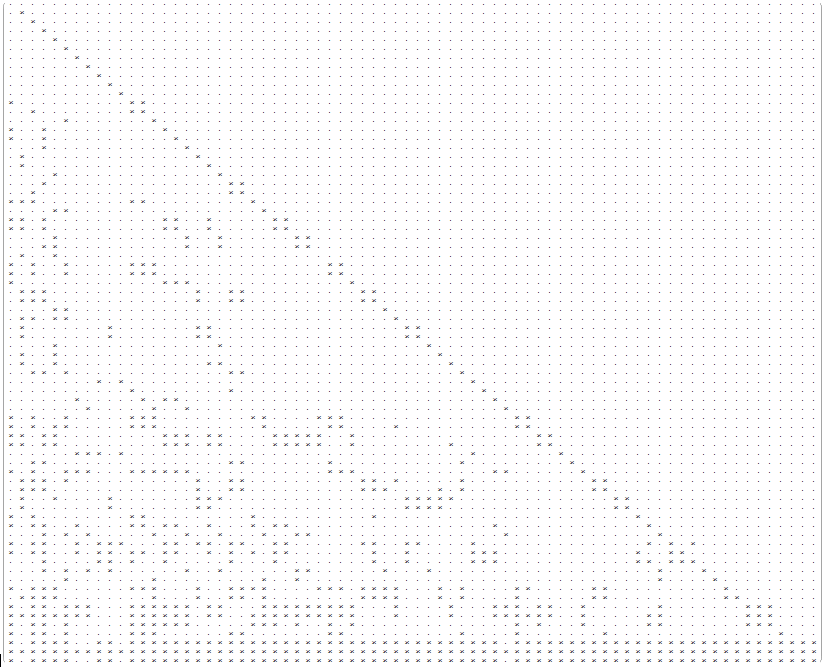
\includegraphics[width=0.8\pagewidth]{img/matrix.png} }
\newpage


\titleb{Example 1}{Epsilon Form by \fuchsia}
Let us introduce a new variable $y$, such that
$$p^2 = -4m^2\frac{y^2}{1-y^2}$$%
The new equations look as
  $$
    \begin{aligned}
     \frac{\D F_1}{\D y} & = 0
     \\
     \frac{\D F_2}{\D y} & = \frac{1-\eps}{y \x m^2} F_1 + \left( \frac{\eps}{1-y} - \frac{\eps}{1+y} - \frac{1}{y} \right) F_2
    \end{aligned}
  $$%
With the help of \fuchsia we find a new basis $G_1$, $G_2$ given by the system
  $$
    \begin{aligned}
     F_1 & = \frac{4(1-2\eps)}{3(1-\eps)} G_1
     \\
     F_2 & = \frac{4}{3m^2} G_1 - \frac{2}{y} G_2
    \end{aligned}
  $$%
For this basis the differential equations are the epsilon form
  $$
    \begin{aligned}
     \frac{\D G_1}{\D y} & = 0
     \\
     \frac{\D G_2}{\D y} & = \frac{2}{3m^2}\left( \frac{\eps}{1+y}+\frac{\eps}{1-y} \right) G_1 - \left(\frac{\eps}{1-y}-\frac{\eps}{1+y}\right) G_2
    \end{aligned}
  $$
\newpage


\titlea{III. Solutions}
We are looking for the solution of a given system of ordinary differential equations in the epsilon form
$$
\frac{\D G}{\D x} = \eps \x B(x) \x G
$$%
as a Laurent series in $\eps$
$$
  \bbox{
  G(x,\eps) = G_0(x) + G_1(x) \x \eps + G_2(x) \x \eps^2 + \ldots}
$$%
Let us put this "solution" into the initial equation
$$
\frac{\D G_0}{\D x} + \frac{\D G_1}{\D x} \eps + \frac{\D G_2}{\D x} \eps^2 + \ldots = \eps \x B(x) \x G_0 + \eps^2 \x B(x) \x G_1
$$%
we get
$$
 \frac{\D G_0}{\D x} = 0,
 \qquad
 \frac{\D G_1}{\D x} = B(x) G_0,
 \qquad
 \frac{\D G_2}{\D x} = B(x) G_1
 \qquad
 \ldots
 \qquad
 \frac{\D G_{n}}{\D x} = B(x) G_{n-1}
$$%
This system can be easily solved (as promised)
$$
 G_0 = C_0,
 \qquad
 G_1 = C_1 + \int \D x B(x) C_0,
 \qquad
 G_2 = C_2 + \int \D x B(x) \left( C_1 + \int \D x B(x) C_0\right)
 \qquad
 \ldots
$$
$$
\bbox{
 G_n(x) = C_n + \int \D x B(x) G_{n-1}
}
$$
\newpage


\titlea{III. Solutions}

My implementation of the solution algorithm, which I use to get results for the next slide.
\vs

\begin{codeblock}
  SolveODE[m_, x_, ep_, n_, c_] := Module[
    {$i, $j, $n, $sol, $sol0, $sol1},

    $n = Length[m];
    $sol[0] = Table[c[$j,0], {$j,1,$n}];
    For[$i=1, $i<=n, $i++,
      $sol0 = Table[c[$j,$i], {$j,1,$n}];
      $sol1 = Integrate[Dot[#,$sol[$i-1]],x]& /@ m;
      $sol[$i] = $sol0 + $sol1;
    ];
    Sum[ep^$i*$sol[$i], {$i,0,n}]
  ];
\end{codeblock}
\newpage


\titleb{Example 1}{Solutions}
\bi
  \item Master \#1
    $$ F_1(y,m^2) = \frac{4}{3}C_1^{(0)} +  \frac{4}{3}\left(C_1^{(1)}-C_1^{(0)}\right)\eps + \ldots $$
  \item Master \#2
    $$
      F_2(y,m^2)
      =
      \frac{4C_1^{(0)}}{3m^2}
      -
      \frac{C_2^{(0)}}{y}
      +
      \frac{\eps}{3m^2y}
      \left(
          4yC_1^{(1)}
        - 6m^2C_2^{(1)}
        + \big(4 C_1^{(1)}
        - 6 m^2 C_2^{(0)}\big) \ln\left(\frac{1-y}{1+y}\right)
      \right)
    $$
  \item Finally, we need to find unknown integration constants whcih are \\ functions of $m^2$ and~$\eps$, i.e.
        $$ C_1^{(0)}(m^2,\eps), \quad  C_1^{(1)}(m^2,\eps), \quad \ldots $$
        $$ C_2^{(0)}(m^2,\eps), \quad  C_2^{(1)}(m^2,\eps), \quad \ldots $$
\ei
\newpage


\titleb{Example 1}{Integration Constants \#1}
    Master \#1 (from \fuchsia)
    $$ F_1(y,m^2) = \frac{4}{3}C_1^{(0)} +  \frac{4}{3}\left(C_1^{(1)}-C_1^{(0)}\right)\eps + \ldots $$

    Closed-form solution from the literature (see Smirnov's book)
    $$ F(0,n) = (-1)^n \frac{\Gamma(n-2+\eps)}{\Gamma(n)} \x (m^2)^{2-\eps-n} $$
    $$
      F_1(y,m^2)
       = F(0,1) 
       = \frac{m^2}{\eps} + m^2 \left(1- \gamma_E - \ln{m^2} \right) + \ldots
    $$

Result \#1
    $$ \bbox{C_1^{(0)} = \frac{3m^2}{4\eps} \quad C_1^{(1)} = \frac{3m^2 \left(2- \gamma_E - \ln{m^2} \right)}{4\eps}}$$
\newpage


\titleb{Example 1}{Integration Constants \#2}
  Result \#1
    $$ C_1^{(0)} = \frac{m^2}{\eps} \quad C_1^{(1)} = \frac{m^2 \left(1- \gamma_E - \ln{m^2} \right)}{\eps}$$

  Master \#2 (with Result \#1 substituted)
    $$
      F_2(y,m^2)
      =
      \frac{1}{\eps}
      +
      \frac{2y - \gamma_E\x y - 2 C_2^{(0)} - y\x \ln{m^2} + \ln\left(\frac{1-y}{1+y}\right)}{y}
      +
      \ldots
    $$

  We require that at the limit $y\to 0$ ($p^2\to 0$) our result is regular. This leads to the solution
$$ C_2^{0} = 0 $$

Result \#2
$$\bbox{
  F_2(y,m^2)
  =
  \frac{1}{\eps}
  +
 2 - \gamma_E\x - \ln{m^2} + \frac{1}{y}\ln\left(\frac{1-y}{1+y}\right)
  +
  \ldots}
$$

This is in agreement with T.Riemann Monday's lecture!
\newpage


\titleb{Example 1}{Summary}
We have seen how to
\bi
  \item generate IBP rules for a given graph
  \item construct differential equations
  \item find epsilon form
  \item solve differential equations
  \item find integration constants
\ei

\fbox{Exercies}
\bi
  \item using \litered choose some two-loop (massless and massive) propagator \\ and find corresponding masters
  \item solve Example \#1, but using equations in $m^2$ (for help see Smirnov's book)
\ei

\newpage


\titleb{Example 2}{Splitting Functions from $e^+ e^-$-annihilation}
In this example, I will show how to calculate a gluon-quark splitting function
$$P_{gq} = \frac{1 + (1-x)^2}{x}$$%
Using this technique you will be able to calculate remaining splitting functions $P_{qq}$, $P_{qg}$, and $P_{gg}$ as well as higher-order corrections to these quantities.
\begin{center}
\begin{axopicture}(300,65)
  \SetScale{0.65}
  \Line[arrow](60,50)(20,90)
  \Line[arrow](20,10)(60,50)
  \Vertex(60,50){2}
  \Photon(60,50)(120,50){5}{4}
  \Vertex(120,50){2}
  \Line[arrow](120,50)(160,90)
  \Line[arrow](160,10)(120,50)
  \Gluon(130,60)(160,60){-4}{3}
  \Vertex(130,60){2}
  \Text(90,65){$q$}
  \Text(10,90){$q_1$}
  \Text(10,10){$q_2$}
  \Text(170,90){$p_1$}
  \Text(170,60){$p_3$}
  \Text(170,10){$p_2$}

  \SetOffset(180,0)
  \Line[arrow](60,50)(20,90)
  \Line[arrow](20,10)(60,50)
  \Vertex(60,50){2}
  \Photon(60,50)(120,50){5}{4}
  \Vertex(120,50){2}
  \Line[arrow](120,50)(160,90)
  \Line[arrow](160,10)(120,50)
  \Gluon(130,40)(160,40){-4}{3}
  \Vertex(130,40){2}
  \Text(90,65){$q$}
  \Text(10,90){$q_1$}
  \Text(10,10){$q_2$}
  \Text(170,90){$p_1$}
  \Text(170,40){$p_3$}
  \Text(170,10){$p_2$}
\end{axopicture}
\end{center}
$$e^+(q_1) + e^-(q_2) \to q(p_1) + \bar{q}(p_2) + g(p_3)$$%
Mass-factorization theorem 
$$
 \frac{\D\sigma_i}{\D x} = \frac{P_{iq}}{\eps} + a_i + b_i \eps + \ldots
$$%
where $q=q_1+q_2$ and
$$
\frac{\D\sigma_i}{\D x} = \int \D^n p_1 \delta(p_1^2) \x \D^n p_2 \delta(p_2^2) \x \D^n p_3 \delta(p_3^2) \x \delta\left(x-\frac{2 q\!\cdot\!p_i}{q^2}\right) \x \sigma(q_1,q_2,p_1,p_2,p_3)
$$
\newpage


\titleb{Example 2}{Phase-Space Integrals}
By their structure phase-space integrals are very similar to loop integrals (compare to the one-loop propagator from Example I), except that we apply on-shell conditions $\delta(p_i^2)$ to the cut lines as shown in the following {\bf cut graph}

\begin{center}
\begin{axopicture}(220,80)
  \SetScale{0.75}
  \Photon(80,50)(120,50){5}{3}
  \Vertex(120,50){2}
  \Line[arrow](160,90)(120,50)
  \Line[arrow](120,50)(160,10)
  \Gluon(130,60)(190,60){-4}{6}
  \Vertex(130,60){2}
  \Vertex(190,60){2}
  \Line[arrow](200,50)(160,90)
  \Line[arrow](160,10)(200,50)
  \Vertex(200,50){2}
  \Photon(200,50)(240,50){5}{3}
  \DashLine(160,5)(160,95){6}
\end{axopicture}
\end{center}

$$
\frac{\D\sigma_g}{\D x} = \int \D^n p_1 \delta(p_1^2) \x \D^n p_2 \delta(p_2^2) \x \D^n p_3 \delta(p_3^2) \x \delta\left(x-\frac{2 q\!\cdot\!p_3}{q^2}\right) \x \sigma(q_1,q_2,p_1,p_2,p_3)
$$
where
$$
\sigma(q_1,q_2,p_1,p_2,p_3)
=
N \frac{(\spr{p_1}{q_1})^2+(\spr{p_2}{q_1})^2+(\spr{p_1}{q_2})^2+(\spr{p_2}{q_2})^2}{\spr{p_1}{p_3}\x\spr{p_2}{p_3}}
$$
This integration is equivalent to the 2-loop propagator, since we can eliminate one of the integration momenta using momentum conservation
$$ q_1 + q_2 = p_1 + p_2 + p_3 $$
\newpage


\titleb{Example 2}{Integration by Parts}

In order to integrate the cross-section we need a new IBP basis. Let us define one as
\vs

\begin{codeblock}
NewBasis[$a,{sp[p1], sp[p3], sp[q1+q2-p1-p3], s*x-2sp[q1+q2,p3], sp[p1,p3]},
            {p1, p3}, Append -> True];

GenerateIBP[$a];
AnalyzeSectors[$a, {___,0,0}, CutDs -> {1,1,1,1,0,0,0}];
FindSymmetries[];

SolvejRules /@ UniqueSectors[$a];
\end{codeblock}
\vs
Note additional arguments in \code{AnalyzeSectors} routine:
\bi
  \item in \code{\{\_\_\_,0,0\}} 0's represent invariants which appear in numerators only
  \item in \code{CutDs -> \{1,1,1,1,0,0,0\}} 1's represent "cut" propagators. It means that all integrals with at least one non-positive indices in these places vanish.
\ei

\vs
We get only one master integral
$$
F_1(x,\eps) = \int \D^n p_1 \delta(p_1^2) \x \D^n p_2 \delta(p_2^2) \x \D^n p_3 \delta(p_3^2) \x \delta\left(x-\frac{2 q\!\cdot\!p_3}{q^2}\right)
$$
\newpage


\titlea{IV. Partial Fractioning}
Given a set of denominators, being a {\em linear combination} of the kinematic invariants $s_{ij}$, make a partial fraction such that
$$
  \frac{1}{D_1\ldots D_n} \to \frac{a_1}{D_2 \ldots D_n} +  \frac{a_2}{D_1 D_3 \ldots D_n} + \ldots + \frac{a_n}{D_1 \ldots D_{n-1}}
$$

All we need is to solve a linear system of equations
$$ a_1 D_1 + \ldots + a_n D_n = N $$
where the coefficient in front of every $s_{ij}$ is zero and $N$ is some number.

\vs
In particaulr, for
$$
  A = \frac{1}{(x+1)(y+1)(x+y+1)}
$$
we write down
$$
  (a_1 + a_3) x + (a_2 + a_3) y + a_1 + a_2 + a_3 = N
$$
the solution is
$$
  a_1 = - a_3 \quad  a_2 = - a_3 \quad N = - a_3
$$
which gives
$$
  A = \frac{1}{(y+1)(x+y+1)} + \frac{1}{(x+1)(x+y+1)} - \frac{1}{(x+1)(y+1)}
$$
\newpage


\titleb{Example 2}{IBP Reduction}
Now we can convert the initial cross-section into the $j$-form and make IBP reduction.
\vs

\begin{codeblock}
M2 = (sp[p1,q1]^2+sp[p1,q2]^2+sp[p2,q1]^2+sp[p2,q2]^2)/(x*sp[q1,q2]*sp[p1,p3])

PS2 = x / (sp[p1]*sp[p3]*sp[q1+q2-p1-p3]*(s*x-2*sp[q1+q2,p3]));

jM2 = Toj[$a, PS2*M2];

jM2 = jM2 // IBPReduce

Pgq = Series[jM2 /. {m -> 4-2*eps}, {eps, 0, -1}]
\end{codeblock}
\vs
This gives us
$$ P_{gq} \sim \frac{2-2x+x^2}{\color{red}x^2} \x F_1(x)  $$%
which contains one $x$ factor more in the denominator than we expect.

\vs\vs
Maybe $F_1(x) \sim x$? Let us check\ldots

\newpage


\titleb{Example 2}{Differential Equations}
\begin{codeblock}
F1 = j[$a, 1, 1, 1, 1, 0, 0, 0];

dF1 = Toj[$a, D[Fromj[$F1], x]] // IBPReduce;
\end{codeblock}
\vs
This code produces the following equation
$$
  \frac{\D F_1}{\D x} = \left( \frac{\eps}{1-x}+\frac{1-2\eps}{x} \right) F_1
$$

Of course we could use \fuchsia and find the $\eps$-form, but we can solve this in a closed form
$$
  F_1 = C(\eps) \x (1-x)^\eps \x x^{1-2\eps}
$$
which confirms our assumption from the previous slide.

The final result is
$$ \bbox{P_{gq} \sim \frac{2-2x+x^2}{x}}$$%
\newpage


\titleb{Example 2}{Summary}
Now you also now how to calculate phase-space integrals.

\vs\vs
\fbox{Exercise}\par
Redefine $x$ as
$$x = \frac{2\spr{q}{p_1}}{q^2}$$
and find a well-known result
$$ P_{qq} = \frac{1+x^2}{1-x} $$
 for the quark-quark splitting function.
\newpage


\titlea{V. Holonomic Functions}
A function $f=f(x)$ is called {\em holonomic} if there exist polynomials $a_n(x),\x\ldots,\x a_0(x)$ such that
$$
  \label{eq:ode}
  a_n(x) f^{(n)} - a_{n-1}(x)\x f^{(n-1)} - \ldots - a_0(x) \x f = 0
$$%
holds for all $x$. Hence, the holonomic function is uniquely defined by
\bi
  \item the differential equation
  \item a number of initial values $f(x_0),\x f'(x_0),\x \ldots,\x f^{(n-1)}(x_0)$
\ei

\vs
\underline{Examples} of holonomic functions:
\bi
  \item {\em all algebraic functions}
  \item \fbox{\em Generalized Hypergeometric functions}
    \bi
      \item {\em polylogarythms}
      \item {\em Elliptic functions}
    \ei
  \item {\em Bessel functions}
  \item {\em Airy functions}
  \item {\em Legendre and Chebyshev polynomials}
  \item {\em Heun functions}
  \item and many others that have no name and no closed form
\ei
\newpage

\titlea{V. Holonomic Functions}
A function $f=f(x)$ is called {\em holonomic} if there exist polynomials $a_n(x),\x\ldots,\x a_0(x)$ such that
$$
  a_n(x) f^{(n)} - a_{n-1}(x)\x f^{(n-1)} - \ldots - a_0(x) \x f = 0
$$%
holds for all $x$. Hence, the holonomic function is uniquely defined by
\bi
  \item the differential equation
  \item a number of initial values $f(x_0),\x f'(x_0),\x \ldots,\x f^{(n-1)}(x_0)$
\ei


\vs
\underline{Conclusion}
\bi
  \item simple representation
  \bi
    \item polynomials
    \item ordinary differential equations
  \ei
  \item define many complicated functions
  \bi
    \item no closed form
    \item non-trivial integration representation
  \ei
  \item represent Feynman integrals
  \item alternative for direct integration
\ei
\newpage


\titlea{V. Holonomic Functions}

We can easily rewrite a $n^{\text{th}}$-order linear ODE given by
\be
  \label{eq:ode}
  y^{(n)} - a_1(x)\x y^{(n-1)} - \ldots - a_n(x) \x y = 0
\ee
as an $n\times n$ system of the form 
$$ \frac{\D \bar{y}}{\D x} = A(x) \x \bar{y} $$%
where
$$
A(x) =
\begin{bmatrix}
  0 & 1 & \cdots & 0 & 0
  \\
  0 & 0 & \cdots & 0 & 0
  \\
  \vdots & \vdots & \ddots & \vdots & \vdots
  \\
  0 & 0 & \cdots & 0 & 1
  \\
  a_n(x) & a_{n-1}(x) & \cdots & a_2(x) & a_1(x)
\end{bmatrix}
\quad \text{and} \quad
\bar{y} =
\begin{pmatrix}
  y \\ y' \\ \vdots \\ y^{(n-2)} \\ y^{(n-1)}
 \end{pmatrix}
$$%
However, the inverse opperation is not as easy anymore.
\newpage


\titlea{VI. Hypergeometric Functions}
The Generalized Hypergeometric Function
$$
 _{p+1}F_p
\left(
\begin{matrix}
  a_1,\x a_2,\x \ldots,\x a_{p+1}
  \\
  b_1,\x b_2,\x \ldots,\x b_{p}
\end{matrix}
;\x x
\right)
=
\prod_{i=1}^{p}\frac{\Gamma(b_i)}{\Gamma(a_i)\Gamma(b_i-a_i)}
\int_0^1 \frac{t_i^{a_i-1} (1-t_i)^{b_i-a_i-1}}{(1-x\x t_1\ldots t_{p})^{a_{p+1}}} \D t_i
$$%
is a solution to the differential equation
$$
\left[
 D \x (D+b_1-1)\x\cdots\x(D+b_p-1)\x - \x x\x(D+a_1)\x\cdots\x(D+a_{p+1})
\right] \x y = 0
$$%
where
$$D = x\frac{\D}{\D x}$$

\vs
\fbox{Exercise}\par
Using your favourite CAS write a routine which for a given Generalized Hypergeometric Function, defined by the list $\{a_1,\ldots,a_{p+1},b_1,\ldots,b_p\}$, returns a corresponding ODE, defined by the list $\{a_1(x),\ldots,a_p(x)\}$, in accordance with notation of eq.~\eqref{eq:ode}.

\newpage


\titlea{Reading List}
\bi \item \people{Feynman Integral Calculus} by V.~Smirnov
    \item \people{Lectures on Differential Equations for Feynman Integrals} by J.~Henn
    \item \people{Formal Power Series and Linear Systems of \\ Meromorphic Ordinary Differential Equations} by W.~Balser
    \item \people{Computer Algebra in Particle Physics} by S.~Weinzierl
    \item \people{Introduction to Loop Calculations} by G.~Heinrich
    \item \people{Structure and Interpretation of Computer Programs}\\by H.~Abelson and G.~Sussman with J.~Sussman
    \ei

\end{document}
